\section{METODOLOGÍA DE DESARROLLO}

Para garantizar un ciclo de vida estructurado, reproducible y alineado con los estándares internacionales de la ciencia de datos, el proyecto adopta una adaptación de la metodología estándar **CRISP-DM** (\textit{Cross-Industry Standard Process for Data Mining}), combinada con los lineamientos de **ASUM-DM** (\textit{Analytics Solutions Unified Method for Data Mining}) orientados a arquitecturas cloud y web contemporáneas. 

El proceso se articula en seis fases secuenciales e iterativas, descritas a continuación y sintetizadas en la Tabla~\ref{tab:fases_metodologia}.

\subsection{Fases de la Metodología Adaptada}

\begin{enumerate}[leftmargin=*, label=\textbf{Fase \arabic*:}]
    \item \textbf{Comprensión del Dominio y Requerimientos Ciudadanos:}  
    Se identificaron las necesidades prioritarias de información en el eje central de Bolivia: monitoreo de precios de alimentos de primera necesidad (supermercados y mercados tradicionales), detección de dispersión de precios en medicamentos esenciales y acceso georreferenciado a establecimientos de salud. Se definieron las métricas clave de ahorro monetario ($\Delta\text{Bs}$) y porcentual ($\Delta\%$).

    \item \textbf{Comprensión y Análisis de los Datos Web:}  
    Se realizó una inspección técnica profunda del DOM, la jerarquía de selectores CSS y los mecanismos de red de cada fuente objetivo:
    \begin{itemize}[leftmargin=*]
        \item \textit{Hipermaxi:} Análisis de la arquitectura SPA Angular, catálogo de 29 sucursales, comportamiento de scroll infinito y respuestas del WAF Radware Bot Manager.
        \item \textit{Farmacorp:} Identificación de 70+ colecciones temáticas en Shopify y mapeo del paginador numérico \texttt{nav.pagination} (Figura~\ref{fig:farmacorp_dom_analisis}).
        \item \textit{Farmacias Chávez:} Decodificación del componente de paginación simple de Ant Design (\texttt{.ant-pagination-simple-pager}) en su interfaz SSR con Next.js (Figura~\ref{fig:chavez_dom_analisis}).
        \item \textit{SICOES:} Mapeo de formularios ASP.NET, estructuras de tablas de convocatorias y descarga de pliegos DBC.
        \item \textit{OpenStreetMap:} Consulta sobre Overpass API para extraer coordenadas geodésicas y metadatos de 83 centros de salud en La Paz.
    \end{itemize}

\begin{figure}[htbp]
    \centering
    \caption{Estructura de Navegación y Paginador Numérico de Farmacorp en Shopify}
    \label{fig:farmacorp_dom_analisis}
    \begin{minipage}{0.48\linewidth}
        \centering
        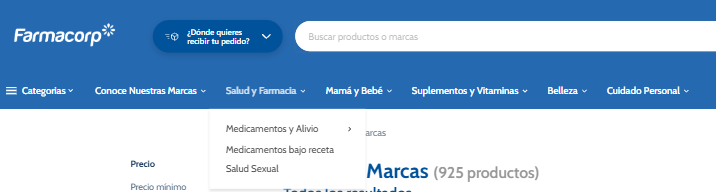
\includegraphics[width=\linewidth]{figuras/farmacorp_taxonomia_categorias.png}
        \caption*{(a) Taxonomía de macro-categorías}
    \end{minipage}\hfill
    \begin{minipage}{0.48\linewidth}
        \centering
        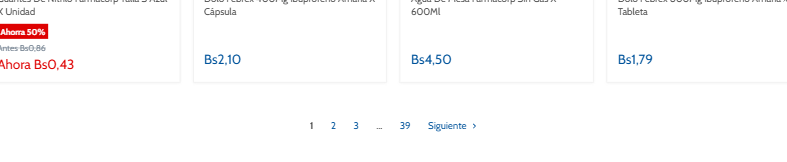
\includegraphics[width=\linewidth]{figuras/farmacorp_paginacion_shopify.png}
        \caption*{(b) Paginador numérico \texttt{nav.pagination}}
    \end{minipage}
    \figurenote{Inspección técnica del DOM de Farmacorp. (a) Organización jerárquica de colecciones temáticas. (b) Componente de paginación numérica tradicional que permite recorrer de forma secuencial las 39+ páginas por categoría.}
\end{figure}

\begin{figure}[htbp]
    \centering
    \caption{Jerarquía de Familias y Paginador Simple Ant Design en Farmacias Chávez}
    \label{fig:chavez_dom_analisis}
    \begin{minipage}{0.32\linewidth}
        \centering
        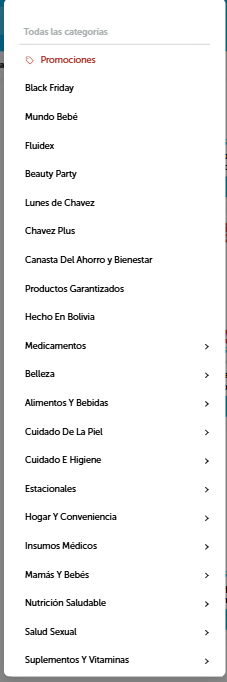
\includegraphics[width=\linewidth]{figuras/chavez_taxonomia_categorias.png}
        \caption*{(a) Menú de categorías}
    \end{minipage}\hfill
    \begin{minipage}{0.65\linewidth}
        \centering
        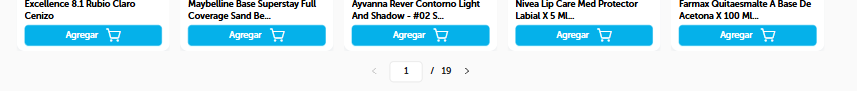
\includegraphics[width=\linewidth]{figuras/chavez_paginacion_ant_design.png}
        \caption*{(b) Paginación compacta \texttt{.ant-pagination-simple-pager}}
    \end{minipage}
    \figurenote{Estructura visual de Farmacias Chávez. (a) Menú lateral con más de 20 familias farmacéuticas. (b) Control de paginación compacta de Ant Design decodificado mediante expresiones regulares sobre el indicador textual de página total.}
\end{figure}

    \item \textbf{Preparación, Limpieza y Normalización de Datos:}  
    Los datos recolectados presentan inconsistencias léxicas, abreviaturas heterogéneas y formatos numéricos locales (comas decimales, prefijos monetarios ``Bs.''). Se implementó un motor de normalización en Node.js que:
    \begin{itemize}[leftmargin=*]
        \item Estandariza nombres de producto y extrae la unidad de medida (kg, g, L, ml, comprimidos, tabletas).
        \item Clasifica automáticamente medicamentos identificando el principio activo, la presentación y el laboratorio fabricante mediante diccionarios especializados de la industria boliviana (INTI, BAGÓ, COFAR, VITA, etc.).
        \item Genera un identificador canónico unívoco (\texttt{sku\_id}) que permite vincular la misma referencia a través de múltiples observaciones temporales.
    \end{itemize}

    \item \textbf{Modelado y Persistencia en Base de Datos:}  
    Diseño e implementación de un esquema en modelo estrella en Neon Serverless PostgreSQL. Los atributos inmutables residen en \texttt{catalogo\_productos\_master}, mientras que las observaciones dinámicas de precios se almacenan en la tabla particionada mensualmente \texttt{precios\_historico}. Se programaron funciones PL/pgSQL reactivas desacopladas para mantener la integridad referencial lógica y computar variaciones de precio en tiempo de inserción. Asimismo, se generaron embeddings vectoriales de 1024 dimensiones con NVIDIA NIM para las licitaciones públicas de SICOES y se construyó el grafo de contrataciones en \texttt{sicoes\_graph\_edges}.

    \item \textbf{Evaluación, Telemetría y Auditoría Técnica:}  
    Validación rigurosa de los flujos de extracción y cálculo:
    \begin{itemize}[leftmargin=*]
        \item Verificación de tasas de recolección (productos por segundo) y latencias de base de datos en consola (Figura~\ref{fig:telemetria_consola_scroll}).
        \item Auditoría de disparadores reactivos mediante inserciones sintéticas controladas y reversión transparente sin afección de datos reales.
        \item Evaluación de la precisión de búsqueda semántica vectorial frente al motor sintáctico tradicional.
    \end{itemize}

\begin{figure}[htbp]
    \centering
    \caption{Monitoreo en Consola de la Carga Asíncrona por Lotes en Hipermaxi Calacoto}
    \label{fig:telemetria_consola_scroll}
    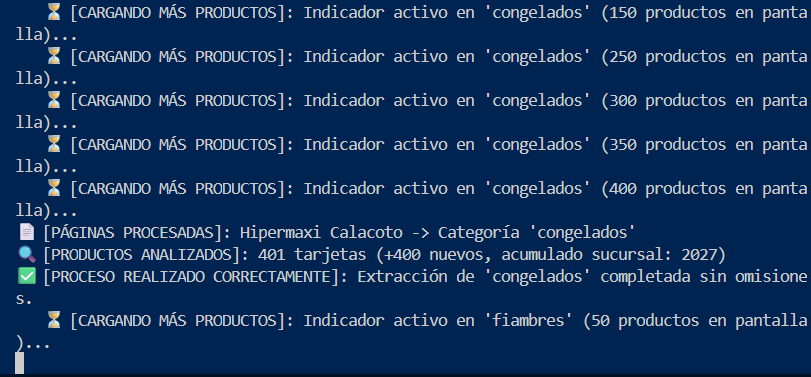
\includegraphics[width=0.88\linewidth]{figuras/imgEjecucionConsola.png}
    \figurenote{Salida en tiempo real del crawler durante el desplazamiento vertical continuo. Ilustra la detección del indicador de carga en lotes sucesivos de 50 productos hasta consolidar 401 tarjetas en la categoría congelados sin pérdida de información.}
\end{figure}

    \item \textbf{Despliegue y Consumo Ciudadano Multiplataforma:}  
    Puesta en producción de dos canales de interacción ciudadana de acceso abierto: el bot conversacional en Telegram (\texttt{@ChatDM7200bot}) con navegación por menús inline y geolocalización Haversine; y la plataforma web interactiva en Next.js 14 provista de dashboards comparativos y cartografía dinámica con Leaflet.
\end{enumerate}

\begin{table}[htbp]
    \centering
    \small
    \caption{Matriz de Fases Metodológicas, Actividades Principales y Entregables del Proyecto}
    \label{tab:fases_metodologia}
    \begin{tabularx}{\linewidth}{>{\raggedright\arraybackslash}p{3.8cm} >{\raggedright\arraybackslash}p{6.2cm} L}
        \toprule
        \textbf{Fase Metodológica} & \textbf{Actividades Principales} & \textbf{Entregables Técnicos} \\
        \midrule
        1. Comprensión del Dominio & Análisis de asimetría de precios, necesidades ciudadanas y alcance geográfico (eje central). & Especificación formal de requerimientos y métricas de variación ($\Delta\text{Bs}$, $\Delta\%$). \\
        \addlinespace
        2. Comprensión de Datos Web & Auditoría DOM, inspección de protocolos de red, evaluación de WAF Radware y selectores. & Diccionario de 700+ selectores, rutas y parámetros de paginación analizados. \\
        \addlinespace
        3. Preparación de Datos & Extracción de unidades, normalización de fármacos (40+ principios activos, 35+ laboratorios). & Motor de limpieza en TypeScript y generador de \nolinkurl{sku_id} canónicos. \\
        \addlinespace
        4. Modelado y Persistencia & Particionamiento mensual, triggers reactivos PL/pgSQL, vectorización NIM y grafos. & Esquema DDL \nolinkurl{schema.sql}, índices HNSW \nolinkurl{pgvector} y tablas de grafos. \\
        \addlinespace
        5. Evaluación y Auditoría & Pruebas de carga, telemetría de consola, pruebas de inyección y verificación de deltas. & Banners de telemetría, validación de integridad y métricas cuantitativas auditadas. \\
        \addlinespace
        6. Despliegue y Difusión & Configuración de webhooks en Telegram y compilación de plataforma web en Next.js 14. & Bot \texttt{@ChatDM7200bot} y plataforma web con mapas OpenStreetMap. \\
        \bottomrule
    \end{tabularx}
    \tablenote{Adaptación del modelo CRISP-DM / ASUM-DM para minería web integral. Describe la trazabilidad desde el análisis inicial de dominio hasta el despliegue multiplataforma en producción.}
\end{table}
